\documentclass[oneside, final, 12pt]{article}

\pagestyle{plain}

\usepackage{a4wide}
\usepackage[utf8]{inputenc}
\usepackage[russian]{babel}
\usepackage{vmargin}
\setpapersize{A4}
\setmarginsrb{2cm}{1.5cm}{1cm}{1.5cm}{5pt}{5mm}{5pt}{13mm}
\usepackage{indentfirst}
\usepackage{graphicx}

\usepackage{amsmath}
\usepackage{amsfonts}
\usepackage{amsthm}
\usepackage{amssymb}

\newcommand{\norm}[1]{\left\lVert #1 \right\rVert}

\newtheorem{definition}{Определение}
\newtheorem{feature}{Свойство}
\newtheorem{statement}{Утверждение}
\newtheorem{sthm}{Теорема}


\begin{document}


\thispagestyle{empty}

\begin{center}
\ \vspace{-3cm}

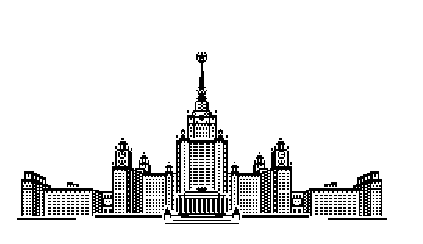
\includegraphics[width=0.5\textwidth]{msu.eps}\\
{\scshape Московский государственный университет имени М.~В.~Ломоносова}\\
Факультет вычислительной математики и кибернетики\\
Кафедра системного анализа

\vfill

\begin{LARGE}
	Отчёт по практикуму

\end{LARGE}

\vspace{1cm}

\begin{Huge}
\bfseries <<Прикладные задачи системного анализа: задачи биоматематики>>

\end{Huge}

\end{center}

\vspace{1cm}

\begin{flushright}
  \large
  \textit{Студентка 515 группы}\\
  А.\,А.~Наумова

  \vspace{5mm}

  \textit{Руководитель практикума}\\
   аспирант Д.\,А.~Алимов

\end{flushright}

\vfill

\begin{center}
Москва, 2020
\end{center}

\newpage
\tableofcontents								%	СОДЕРЖАНИЕ

\newpage
\section{Постановка задачи}						%	ПОСТАНОВКА ЗАДАЧИ
	\[
	\begin{cases}
	\dot{u} = au - \dfrac{bu^2v}{1 + Pu} + d_1u_{xx}, \\
	\dot{v} = -cv + \dfrac{du^2v}{1 + Pu} + d_2v_{xx}.
	\end{cases}
	\]

\newpage
\section{Исследование фазового портрета нераспределенной системы}						%
\subsection{Замена переменных}
Пусть
\[
    \widetilde{u} = \alpha u;\\
    \widetilde{v} = \beta u;\\
    \widetilde{t} = \gamma t;\\
    \widetilde{x} = \delta x.
\]
Тогда система примет следующий вид:
\[
    \begin{cases}
        \dfrac{\gamma}{\alpha} \widetilde{u}_{\widetilde{t}} =
        \dfrac{a}{\alpha}\widetilde{u}
        - \dfrac{b}{\alpha^2\beta} \dfrac{\widetilde{u}^2\widetilde{v}}{(1 + P\widetilde{u}/\alpha)}
        + d_1\dfrac{\delta^2}{\alpha} \widetilde{u}_{\widetilde{x}\widetilde{x}}, \\

        \dfrac{\gamma}{\beta} \widetilde{v}_{\widetilde{t}} =
        \dfrac{-c}{\beta}\widetilde{v}
        + \dfrac{d}{\alpha^2\beta} \dfrac{\widetilde{u}^2\widetilde{v}}{(1 + P\widetilde{u}/\alpha)}
        + d_2\dfrac{\delta^2}{\beta} \widetilde{v}_{\widetilde{x}\widetilde{x}}.
    \end{cases}
\]
Чтобы избавиться от лишних коэффициентов, возьмем
\[
    \gamma = a;\\
    \beta = \dfrac{b}{a};\\
    \alpha = P;\\
    \delta = \sqrt{\dfrac{a}{d_2}}.
\]
Получим
\[
    \begin{cases}
        \dot{u} = u\left(1 - \dfrac{1}{P} \dfrac{uv}{1 + u}\right)  + \dfrac{d_1}{d_2}u_{xx}, \\
        \dot{v} = \dfrac{-c}{a} v\left(1 - \dfrac{d}{P^{2}c} \dfrac{u^2}{1 + u}\right) + v_{xx}.
    \end{cases}
\]
Переобозначим
\[
    k_1 = \dfrac{1}{P};\\
    k_2 = \dfrac{-c}{a};\\
    k_3 = \dfrac{d}{P^{2}c}.
\]
Предполагаем, что \(d_1 = 0\) (жертвы сконцентрированы в одной точке). Тогда получаем систему размерности 3:
\[
    \begin{cases}
        \dot{u} = u\left(1 -  k_1\dfrac{uv}{1 + u}\right) , \\
        \dot{v} = k_2 v\left(1 - k_3 \dfrac{u^2}{1 + u}\right) + v_{xx}.
    \end{cases}
\]

\subsection{Неподвижные точки и их тип}

Якобиан системы имеет вид:\\
J(u,v) =
\begin{pmatrix}
    \(1-k_1 v\left(\dfrac{1}{(1+u)^2}\right)\) & \(-k_1 \dfrac{u^2}{1+u}\)\\
    \(-k_2 k_3 v \dfrac{2u + u^2}{\left( 1+u \right)^2} \) & \(k_2 \left( 1 - k_3\dfrac{u^2}{1+u} \right)\)
\end{pmatrix}\\

Рассмотрим неподвижную точку \( T_1 = (0, 0).\) \\

Якобиан в этой точке принимает вид:
J(0,0) =
\begin{pmatrix}
    1 & 0\\
    0 & k_2
\end{pmatrix}\\

Так как существует собственное значение с положительной вещественной частью (\lambda_1=1\),
то данная точка неустойчива по теореме Ляпунова о неустойчивости по первому приближению.\\

Далее рассмотрим систему уравнений:
\[
    \begin{cases}
        1 -  k_1\dfrac{uv}{1 + u} = 0, \\
        1 - k_3 \dfrac{u^2}{1 + u} = 0.
    \end{cases}
\]\\

Решение второго уравнения: \(u = \dfrac{1 \pm \sqrt{1+4k_3}}{2k_3} \).\\

Так как \(k_3 > 0\), в область \(\cal{R}^+\) попадает только \(u^* = \dfrac{1 + \sqrt{1+4k_3}}{2k_3} \).\\

\(v^* = \dfrac{1+u^*}{k_1 u^*} = \dfrac{1}{k_1} \left( 1 + \dfrac{2k_3}{1 + \sqrt{1+4k_3}} \right) \).\\

Исследуем теперь данную неподвижную точку \( T_2 = (u^*, v^*).\) \\

Якобиан в этой точке принимает вид:\\
J(u*,v*) =
\begin{pmatrix}
    \(1-k_1 \left( \dfrac{1}{k_1} \left( 1 + \dfrac{2k_3}{1 + \sqrt{1+4k_3}} \right) \right)\left(\dfrac{1}{(1+ \left( \dfrac{1 \pm \sqrt{1+4k_3}}{2k_3} \right) )^2}\right)\) & \(-k_1 \dfrac{\left( \dfrac{1 \pm \sqrt{1+4k_3}}{2k_3} \right)^2}{1+\left( \dfrac{1 \pm \sqrt{1+4k_3}}{2k_3} \right)}\)\\
    \(-k_2 k_3 \left( \dfrac{1}{k_1} \left( 1 + \dfrac{2k_3}{1 + \sqrt{1+4k_3}} \right) \right) \dfrac{ \left( \dfrac{1 \pm \sqrt{1+4k_3}}{2k_3} \right) \left( 2 + \left( \dfrac{1 \pm \sqrt{1+4k_3}}{2k_3} \right) \right)}{\left( 1+\left( \dfrac{1 \pm \sqrt{1+4k_3}}{2k_3} \right) \right)^2} \) & \(k_2 \left( 1 - k_3\dfrac{\left( \dfrac{1 \pm \sqrt{1+4k_3}}{2k_3} \right)^2}{1+\left( \dfrac{1 \pm \sqrt{1+4k_3}}{2k_3} \right)} \right)\)
\end{pmatrix}\\

Eugenvalues:\\

\(
\left\{ - \frac{\sqrt{\frac{- 2 k_{2} \left(k_{3}^{2} \sqrt{4 k_{3} + 1} + 5 k_{3}^{2} + 3 k_{3} \sqrt{4 k_{3} + 1} + 5 k_{3} + \sqrt{4 k_{3} + 1} + 1\right)^{2} \left(k_{3}^{13} \sqrt{4 k_{3} + 1} + 27 k_{3}^{13} + 91 k_{3}^{12} \sqrt{4 k_{3} + 1} + 819 k_{3}^{12} + 1365 k_{3}^{11} \sqrt{4 k_{3} + 1} + 7371 k_{3}^{11} + 8008 k_{3}^{10} \sqrt{4 k_{3} + 1} + 30888 k_{3}^{10} + 24310 k_{3}^{9} \sqrt{4 k_{3} + 1} + 72930 k_{3}^{9} + 43758 k_{3}^{8} \sqrt{4 k_{3} + 1} + 107406 k_{3}^{8} + 50388 k_{3}^{7} \sqrt{4 k_{3} + 1} + 104652 k_{3}^{7} + 38760 k_{3}^{6} \sqrt{4 k_{3} + 1} + 69768 k_{3}^{6} + 20349 k_{3}^{5} \sqrt{4 k_{3} + 1} + 32319 k_{3}^{5} + 7315 k_{3}^{4} \sqrt{4 k_{3} + 1} + 10395 k_{3}^{4} + 1771 k_{3}^{3} \sqrt{4 k_{3} + 1} + 2277 k_{3}^{3} + 276 k_{3}^{2} \sqrt{4 k_{3} + 1} + 324 k_{3}^{2} + 25 k_{3} \sqrt{4 k_{3} + 1} + 27 k_{3} + \sqrt{4 k_{3} + 1} + 1\right) \left(2 k_{3}^{22} \sqrt{4 k_{3} + 1} + 88 k_{3}^{22} + 484 k_{3}^{21} \sqrt{4 k_{3} + 1} + 7106 k_{3}^{21} + 19481 k_{3}^{20} \sqrt{4 k_{3} + 1} + 171787 k_{3}^{20} + 311696 k_{3}^{19} \sqrt{4 k_{3} + 1} + 1965304 k_{3}^{19} + 2643850 k_{3}^{18} \sqrt{4 k_{3} + 1} + 12978900 k_{3}^{18} + 13748020 k_{3}^{17} \sqrt{4 k_{3} + 1} + 55276130 k_{3}^{17} + 47805615 k_{3}^{16} \sqrt{4 k_{3} + 1} + 162806535 k_{3}^{16} + 117675360 k_{3}^{15} \sqrt{4 k_{3} + 1} + 347677200 k_{3}^{15} + 213286590 k_{3}^{14} \sqrt{4 k_{3} + 1} + 556598160 k_{3}^{14} + 292746300 k_{3}^{13} \sqrt{4 k_{3} + 1} + 684241950 k_{3}^{13} + 310465155 k_{3}^{12} \sqrt{4 k_{3} + 1} + 657218445 k_{3}^{12} + 258048960 k_{3}^{11} \sqrt{4 k_{3} + 1} + 499268640 k_{3}^{11} + 169695240 k_{3}^{10} \sqrt{4 k_{3} + 1} + 302366064 k_{3}^{10} + 88763664 k_{3}^{9} \sqrt{4 k_{3} + 1} + 146594536 k_{3}^{9} + 36984860 k_{3}^{8} \sqrt{4 k_{3} + 1} + 56926540 k_{3}^{8} + 12243264 k_{3}^{7} \sqrt{4 k_{3} + 1} + 17646816 k_{3}^{7} + 3196578 k_{3}^{6} \sqrt{4 k_{3} + 1} + 4332552 k_{3}^{6} + 649572 k_{3}^{5} \sqrt{4 k_{3} + 1} + 830946 k_{3}^{5} + 100529 k_{3}^{4} \sqrt{4 k_{3} + 1} + 121771 k_{3}^{4} + 11440 k_{3}^{3} \sqrt{4 k_{3} + 1} + 13160 k_{3}^{3} + 902 k_{3}^{2} \sqrt{4 k_{3} + 1} + 988 k_{3}^{2} + 44 k_{3} \sqrt{4 k_{3} + 1} + 46 k_{3} + \sqrt{4 k_{3} + 1} + 1\right) + \left(2 k_{3}^{9} + 9 k_{3}^{8} \sqrt{4 k_{3} + 1} + 81 k_{3}^{8} + 120 k_{3}^{7} \sqrt{4 k_{3} + 1} + 540 k_{3}^{7} + 462 k_{3}^{6} \sqrt{4 k_{3} + 1} + 1386 k_{3}^{6} + 792 k_{3}^{5} \sqrt{4 k_{3} + 1} + 1782 k_{3}^{5} + 715 k_{3}^{4} \sqrt{4 k_{3} + 1} + 1287 k_{3}^{4} + 364 k_{3}^{3} \sqrt{4 k_{3} + 1} + 546 k_{3}^{3} + 105 k_{3}^{2} \sqrt{4 k_{3} + 1} + 135 k_{3}^{2} + 16 k_{3} \sqrt{4 k_{3} + 1} + 18 k_{3} + \sqrt{4 k_{3} + 1} + 1\right) \left(- k_{3}^{16} \sqrt{4 k_{3} + 1} - 27 k_{3}^{16} - 89 k_{3}^{15} \sqrt{4 k_{3} + 1} - 759 k_{3}^{15} - 1140 k_{3}^{14} \sqrt{4 k_{3} + 1} - 5116 k_{3}^{14} - 3808 k_{3}^{13} \sqrt{4 k_{3} + 1} - 5576 k_{3}^{13} + 6630 k_{3}^{12} \sqrt{4 k_{3} + 1} + 60554 k_{3}^{12} + 75582 k_{3}^{11} \sqrt{4 k_{3} + 1} + 293930 k_{3}^{11} + 226746 k_{3}^{10} \sqrt{4 k_{3} + 1} + 659566 k_{3}^{10} + 381140 k_{3}^{9} \sqrt{4 k_{3} + 1} + 912152 k_{3}^{9} + 415701 k_{3}^{8} \sqrt{4 k_{3} + 1} + 853347 k_{3}^{8} + 312455 k_{3}^{7} \sqrt{4 k_{3} + 1} + 563937 k_{3}^{7} + 166474 k_{3}^{6} \sqrt{4 k_{3} + 1} + 268686 k_{3}^{6} + 63480 k_{3}^{5} \sqrt{4 k_{3} + 1} + 92780 k_{3}^{5} + 17225 k_{3}^{4} \sqrt{4 k_{3} + 1} + 23023 k_{3}^{4} + 3249 k_{3}^{3} \sqrt{4 k_{3} + 1} + 4003 k_{3}^{3} + 405 k_{3}^{2} \sqrt{4 k_{3} + 1} + 463 k_{3}^{2} + 30 k_{3} \sqrt{4 k_{3} + 1} + 32 k_{3} + \sqrt{4 k_{3} + 1} + 1\right)^{2}}{2 k_{3}^{9} + 9 k_{3}^{8} \sqrt{4 k_{3} + 1} + 81 k_{3}^{8} + 120 k_{3}^{7} \sqrt{4 k_{3} + 1} + 540 k_{3}^{7} + 462 k_{3}^{6} \sqrt{4 k_{3} + 1} + 1386 k_{3}^{6} + 792 k_{3}^{5} \sqrt{4 k_{3} + 1} + 1782 k_{3}^{5} + 715 k_{3}^{4} \sqrt{4 k_{3} + 1} + 1287 k_{3}^{4} + 364 k_{3}^{3} \sqrt{4 k_{3} + 1} + 546 k_{3}^{3} + 105 k_{3}^{2} \sqrt{4 k_{3} + 1} + 135 k_{3}^{2} + 16 k_{3} \sqrt{4 k_{3} + 1} + 18 k_{3} + \sqrt{4 k_{3} + 1} + 1}}}{\left(k_{3}^{2} \sqrt{4 k_{3} + 1} + 5 k_{3}^{2} + 3 k_{3} \sqrt{4 k_{3} + 1} + 5 k_{3} + \sqrt{4 k_{3} + 1} + 1\right) \left(k_{3}^{13} \sqrt{4 k_{3} + 1} + 27 k_{3}^{13} + 91 k_{3}^{12} \sqrt{4 k_{3} + 1} + 819 k_{3}^{12} + 1365 k_{3}^{11} \sqrt{4 k_{3} + 1} + 7371 k_{3}^{11} + 8008 k_{3}^{10} \sqrt{4 k_{3} + 1} + 30888 k_{3}^{10} + 24310 k_{3}^{9} \sqrt{4 k_{3} + 1} + 72930 k_{3}^{9} + 43758 k_{3}^{8} \sqrt{4 k_{3} + 1} + 107406 k_{3}^{8} + 50388 k_{3}^{7} \sqrt{4 k_{3} + 1} + 104652 k_{3}^{7} + 38760 k_{3}^{6} \sqrt{4 k_{3} + 1} + 69768 k_{3}^{6} + 20349 k_{3}^{5} \sqrt{4 k_{3} + 1} + 32319 k_{3}^{5} + 7315 k_{3}^{4} \sqrt{4 k_{3} + 1} + 10395 k_{3}^{4} + 1771 k_{3}^{3} \sqrt{4 k_{3} + 1} + 2277 k_{3}^{3} + 276 k_{3}^{2} \sqrt{4 k_{3} + 1} + 324 k_{3}^{2} + 25 k_{3} \sqrt{4 k_{3} + 1} + 27 k_{3} + \sqrt{4 k_{3} + 1} + 1\right)} + \frac{- k_{3}^{16} \sqrt{4 k_{3} + 1} - 27 k_{3}^{16} - 89 k_{3}^{15} \sqrt{4 k_{3} + 1} - 759 k_{3}^{15} - 1140 k_{3}^{14} \sqrt{4 k_{3} + 1} - 5116 k_{3}^{14} - 3808 k_{3}^{13} \sqrt{4 k_{3} + 1} - 5576 k_{3}^{13} + 6630 k_{3}^{12} \sqrt{4 k_{3} + 1} + 60554 k_{3}^{12} + 75582 k_{3}^{11} \sqrt{4 k_{3} + 1} + 293930 k_{3}^{11} + 226746 k_{3}^{10} \sqrt{4 k_{3} + 1} + 659566 k_{3}^{10} + 381140 k_{3}^{9} \sqrt{4 k_{3} + 1} + 912152 k_{3}^{9} + 415701 k_{3}^{8} \sqrt{4 k_{3} + 1} + 853347 k_{3}^{8} + 312455 k_{3}^{7} \sqrt{4 k_{3} + 1} + 563937 k_{3}^{7} + 166474 k_{3}^{6} \sqrt{4 k_{3} + 1} + 268686 k_{3}^{6} + 63480 k_{3}^{5} \sqrt{4 k_{3} + 1} + 92780 k_{3}^{5} + 17225 k_{3}^{4} \sqrt{4 k_{3} + 1} + 23023 k_{3}^{4} + 3249 k_{3}^{3} \sqrt{4 k_{3} + 1} + 4003 k_{3}^{3} + 405 k_{3}^{2} \sqrt{4 k_{3} + 1} + 463 k_{3}^{2} + 30 k_{3} \sqrt{4 k_{3} + 1} + 32 k_{3} + \sqrt{4 k_{3} + 1} + 1}{\left(k_{3}^{2} \sqrt{4 k_{3} + 1} + 5 k_{3}^{2} + 3 k_{3} \sqrt{4 k_{3} + 1} + 5 k_{3} + \sqrt{4 k_{3} + 1} + 1\right) \left(k_{3}^{13} \sqrt{4 k_{3} + 1} + 27 k_{3}^{13} + 91 k_{3}^{12} \sqrt{4 k_{3} + 1} + 819 k_{3}^{12} + 1365 k_{3}^{11} \sqrt{4 k_{3} + 1} + 7371 k_{3}^{11} + 8008 k_{3}^{10} \sqrt{4 k_{3} + 1} + 30888 k_{3}^{10} + 24310 k_{3}^{9} \sqrt{4 k_{3} + 1} + 72930 k_{3}^{9} + 43758 k_{3}^{8} \sqrt{4 k_{3} + 1} + 107406 k_{3}^{8} + 50388 k_{3}^{7} \sqrt{4 k_{3} + 1} + 104652 k_{3}^{7} + 38760 k_{3}^{6} \sqrt{4 k_{3} + 1} + 69768 k_{3}^{6} + 20349 k_{3}^{5} \sqrt{4 k_{3} + 1} + 32319 k_{3}^{5} + 7315 k_{3}^{4} \sqrt{4 k_{3} + 1} + 10395 k_{3}^{4} + 1771 k_{3}^{3} \sqrt{4 k_{3} + 1} + 2277 k_{3}^{3} + 276 k_{3}^{2} \sqrt{4 k_{3} + 1} + 324 k_{3}^{2} + 25 k_{3} \sqrt{4 k_{3} + 1} + 27 k_{3} + \sqrt{4 k_{3} + 1} + 1\right)} : 1
\)\\

value 2:\\
\(
\frac{\sqrt{\frac{- 2 k_{2} \left(k_{3}^{2} \sqrt{4 k_{3} + 1} + 5 k_{3}^{2} + 3 k_{3} \sqrt{4 k_{3} + 1} + 5 k_{3} + \sqrt{4 k_{3} + 1} + 1\right)^{2} \left(k_{3}^{13} \sqrt{4 k_{3} + 1} + 27 k_{3}^{13} + 91 k_{3}^{12} \sqrt{4 k_{3} + 1} + 819 k_{3}^{12} + 1365 k_{3}^{11} \sqrt{4 k_{3} + 1} + 7371 k_{3}^{11} + 8008 k_{3}^{10} \sqrt{4 k_{3} + 1} + 30888 k_{3}^{10} + 24310 k_{3}^{9} \sqrt{4 k_{3} + 1} + 72930 k_{3}^{9} + 43758 k_{3}^{8} \sqrt{4 k_{3} + 1} + 107406 k_{3}^{8} + 50388 k_{3}^{7} \sqrt{4 k_{3} + 1} + 104652 k_{3}^{7} + 38760 k_{3}^{6} \sqrt{4 k_{3} + 1} + 69768 k_{3}^{6} + 20349 k_{3}^{5} \sqrt{4 k_{3} + 1} + 32319 k_{3}^{5} + 7315 k_{3}^{4} \sqrt{4 k_{3} + 1} + 10395 k_{3}^{4} + 1771 k_{3}^{3} \sqrt{4 k_{3} + 1} + 2277 k_{3}^{3} + 276 k_{3}^{2} \sqrt{4 k_{3} + 1} + 324 k_{3}^{2} + 25 k_{3} \sqrt{4 k_{3} + 1} + 27 k_{3} + \sqrt{4 k_{3} + 1} + 1\right) \left(2 k_{3}^{22} \sqrt{4 k_{3} + 1} + 88 k_{3}^{22} + 484 k_{3}^{21} \sqrt{4 k_{3} + 1} + 7106 k_{3}^{21} + 19481 k_{3}^{20} \sqrt{4 k_{3} + 1} + 171787 k_{3}^{20} + 311696 k_{3}^{19} \sqrt{4 k_{3} + 1} + 1965304 k_{3}^{19} + 2643850 k_{3}^{18} \sqrt{4 k_{3} + 1} + 12978900 k_{3}^{18} + 13748020 k_{3}^{17} \sqrt{4 k_{3} + 1} + 55276130 k_{3}^{17} + 47805615 k_{3}^{16} \sqrt{4 k_{3} + 1} + 162806535 k_{3}^{16} + 117675360 k_{3}^{15} \sqrt{4 k_{3} + 1} + 347677200 k_{3}^{15} + 213286590 k_{3}^{14} \sqrt{4 k_{3} + 1} + 556598160 k_{3}^{14} + 292746300 k_{3}^{13} \sqrt{4 k_{3} + 1} + 684241950 k_{3}^{13} + 310465155 k_{3}^{12} \sqrt{4 k_{3} + 1} + 657218445 k_{3}^{12} + 258048960 k_{3}^{11} \sqrt{4 k_{3} + 1} + 499268640 k_{3}^{11} + 169695240 k_{3}^{10} \sqrt{4 k_{3} + 1} + 302366064 k_{3}^{10} + 88763664 k_{3}^{9} \sqrt{4 k_{3} + 1} + 146594536 k_{3}^{9} + 36984860 k_{3}^{8} \sqrt{4 k_{3} + 1} + 56926540 k_{3}^{8} + 12243264 k_{3}^{7} \sqrt{4 k_{3} + 1} + 17646816 k_{3}^{7} + 3196578 k_{3}^{6} \sqrt{4 k_{3} + 1} + 4332552 k_{3}^{6} + 649572 k_{3}^{5} \sqrt{4 k_{3} + 1} + 830946 k_{3}^{5} + 100529 k_{3}^{4} \sqrt{4 k_{3} + 1} + 121771 k_{3}^{4} + 11440 k_{3}^{3} \sqrt{4 k_{3} + 1} + 13160 k_{3}^{3} + 902 k_{3}^{2} \sqrt{4 k_{3} + 1} + 988 k_{3}^{2} + 44 k_{3} \sqrt{4 k_{3} + 1} + 46 k_{3} + \sqrt{4 k_{3} + 1} + 1\right) + \left(2 k_{3}^{9} + 9 k_{3}^{8} \sqrt{4 k_{3} + 1} + 81 k_{3}^{8} + 120 k_{3}^{7} \sqrt{4 k_{3} + 1} + 540 k_{3}^{7} + 462 k_{3}^{6} \sqrt{4 k_{3} + 1} + 1386 k_{3}^{6} + 792 k_{3}^{5} \sqrt{4 k_{3} + 1} + 1782 k_{3}^{5} + 715 k_{3}^{4} \sqrt{4 k_{3} + 1} + 1287 k_{3}^{4} + 364 k_{3}^{3} \sqrt{4 k_{3} + 1} + 546 k_{3}^{3} + 105 k_{3}^{2} \sqrt{4 k_{3} + 1} + 135 k_{3}^{2} + 16 k_{3} \sqrt{4 k_{3} + 1} + 18 k_{3} + \sqrt{4 k_{3} + 1} + 1\right) \left(- k_{3}^{16} \sqrt{4 k_{3} + 1} - 27 k_{3}^{16} - 89 k_{3}^{15} \sqrt{4 k_{3} + 1} - 759 k_{3}^{15} - 1140 k_{3}^{14} \sqrt{4 k_{3} + 1} - 5116 k_{3}^{14} - 3808 k_{3}^{13} \sqrt{4 k_{3} + 1} - 5576 k_{3}^{13} + 6630 k_{3}^{12} \sqrt{4 k_{3} + 1} + 60554 k_{3}^{12} + 75582 k_{3}^{11} \sqrt{4 k_{3} + 1} + 293930 k_{3}^{11} + 226746 k_{3}^{10} \sqrt{4 k_{3} + 1} + 659566 k_{3}^{10} + 381140 k_{3}^{9} \sqrt{4 k_{3} + 1} + 912152 k_{3}^{9} + 415701 k_{3}^{8} \sqrt{4 k_{3} + 1} + 853347 k_{3}^{8} + 312455 k_{3}^{7} \sqrt{4 k_{3} + 1} + 563937 k_{3}^{7} + 166474 k_{3}^{6} \sqrt{4 k_{3} + 1} + 268686 k_{3}^{6} + 63480 k_{3}^{5} \sqrt{4 k_{3} + 1} + 92780 k_{3}^{5} + 17225 k_{3}^{4} \sqrt{4 k_{3} + 1} + 23023 k_{3}^{4} + 3249 k_{3}^{3} \sqrt{4 k_{3} + 1} + 4003 k_{3}^{3} + 405 k_{3}^{2} \sqrt{4 k_{3} + 1} + 463 k_{3}^{2} + 30 k_{3} \sqrt{4 k_{3} + 1} + 32 k_{3} + \sqrt{4 k_{3} + 1} + 1\right)^{2}}{2 k_{3}^{9} + 9 k_{3}^{8} \sqrt{4 k_{3} + 1} + 81 k_{3}^{8} + 120 k_{3}^{7} \sqrt{4 k_{3} + 1} + 540 k_{3}^{7} + 462 k_{3}^{6} \sqrt{4 k_{3} + 1} + 1386 k_{3}^{6} + 792 k_{3}^{5} \sqrt{4 k_{3} + 1} + 1782 k_{3}^{5} + 715 k_{3}^{4} \sqrt{4 k_{3} + 1} + 1287 k_{3}^{4} + 364 k_{3}^{3} \sqrt{4 k_{3} + 1} + 546 k_{3}^{3} + 105 k_{3}^{2} \sqrt{4 k_{3} + 1} + 135 k_{3}^{2} + 16 k_{3} \sqrt{4 k_{3} + 1} + 18 k_{3} + \sqrt{4 k_{3} + 1} + 1}}}{\left(k_{3}^{2} \sqrt{4 k_{3} + 1} + 5 k_{3}^{2} + 3 k_{3} \sqrt{4 k_{3} + 1} + 5 k_{3} + \sqrt{4 k_{3} + 1} + 1\right) \left(k_{3}^{13} \sqrt{4 k_{3} + 1} + 27 k_{3}^{13} + 91 k_{3}^{12} \sqrt{4 k_{3} + 1} + 819 k_{3}^{12} + 1365 k_{3}^{11} \sqrt{4 k_{3} + 1} + 7371 k_{3}^{11} + 8008 k_{3}^{10} \sqrt{4 k_{3} + 1} + 30888 k_{3}^{10} + 24310 k_{3}^{9} \sqrt{4 k_{3} + 1} + 72930 k_{3}^{9} + 43758 k_{3}^{8} \sqrt{4 k_{3} + 1} + 107406 k_{3}^{8} + 50388 k_{3}^{7} \sqrt{4 k_{3} + 1} + 104652 k_{3}^{7} + 38760 k_{3}^{6} \sqrt{4 k_{3} + 1} + 69768 k_{3}^{6} + 20349 k_{3}^{5} \sqrt{4 k_{3} + 1} + 32319 k_{3}^{5} + 7315 k_{3}^{4} \sqrt{4 k_{3} + 1} + 10395 k_{3}^{4} + 1771 k_{3}^{3} \sqrt{4 k_{3} + 1} + 2277 k_{3}^{3} + 276 k_{3}^{2} \sqrt{4 k_{3} + 1} + 324 k_{3}^{2} + 25 k_{3} \sqrt{4 k_{3} + 1} + 27 k_{3} + \sqrt{4 k_{3} + 1} + 1\right)} + \frac{- k_{3}^{16} \sqrt{4 k_{3} + 1} - 27 k_{3}^{16} - 89 k_{3}^{15} \sqrt{4 k_{3} + 1} - 759 k_{3}^{15} - 1140 k_{3}^{14} \sqrt{4 k_{3} + 1} - 5116 k_{3}^{14} - 3808 k_{3}^{13} \sqrt{4 k_{3} + 1} - 5576 k_{3}^{13} + 6630 k_{3}^{12} \sqrt{4 k_{3} + 1} + 60554 k_{3}^{12} + 75582 k_{3}^{11} \sqrt{4 k_{3} + 1} + 293930 k_{3}^{11} + 226746 k_{3}^{10} \sqrt{4 k_{3} + 1} + 659566 k_{3}^{10} + 381140 k_{3}^{9} \sqrt{4 k_{3} + 1} + 912152 k_{3}^{9} + 415701 k_{3}^{8} \sqrt{4 k_{3} + 1} + 853347 k_{3}^{8} + 312455 k_{3}^{7} \sqrt{4 k_{3} + 1} + 563937 k_{3}^{7} + 166474 k_{3}^{6} \sqrt{4 k_{3} + 1} + 268686 k_{3}^{6} + 63480 k_{3}^{5} \sqrt{4 k_{3} + 1} + 92780 k_{3}^{5} + 17225 k_{3}^{4} \sqrt{4 k_{3} + 1} + 23023 k_{3}^{4} + 3249 k_{3}^{3} \sqrt{4 k_{3} + 1} + 4003 k_{3}^{3} + 405 k_{3}^{2} \sqrt{4 k_{3} + 1} + 463 k_{3}^{2} + 30 k_{3} \sqrt{4 k_{3} + 1} + 32 k_{3} + \sqrt{4 k_{3} + 1} + 1}{\left(k_{3}^{2} \sqrt{4 k_{3} + 1} + 5 k_{3}^{2} + 3 k_{3} \sqrt{4 k_{3} + 1} + 5 k_{3} + \sqrt{4 k_{3} + 1} + 1\right) \left(k_{3}^{13} \sqrt{4 k_{3} + 1} + 27 k_{3}^{13} + 91 k_{3}^{12} \sqrt{4 k_{3} + 1} + 819 k_{3}^{12} + 1365 k_{3}^{11} \sqrt{4 k_{3} + 1} + 7371 k_{3}^{11} + 8008 k_{3}^{10} \sqrt{4 k_{3} + 1} + 30888 k_{3}^{10} + 24310 k_{3}^{9} \sqrt{4 k_{3} + 1} + 72930 k_{3}^{9} + 43758 k_{3}^{8} \sqrt{4 k_{3} + 1} + 107406 k_{3}^{8} + 50388 k_{3}^{7} \sqrt{4 k_{3} + 1} + 104652 k_{3}^{7} + 38760 k_{3}^{6} \sqrt{4 k_{3} + 1} + 69768 k_{3}^{6} + 20349 k_{3}^{5} \sqrt{4 k_{3} + 1} + 32319 k_{3}^{5} + 7315 k_{3}^{4} \sqrt{4 k_{3} + 1} + 10395 k_{3}^{4} + 1771 k_{3}^{3} \sqrt{4 k_{3} + 1} + 2277 k_{3}^{3} + 276 k_{3}^{2} \sqrt{4 k_{3} + 1} + 324 k_{3}^{2} + 25 k_{3} \sqrt{4 k_{3} + 1} + 27 k_{3} + \sqrt{4 k_{3} + 1} + 1\right)} : 1\right\}

\)
\newpage
\clearpage
\begin{thebibliography}{0}
\addcontentsline{toc}{section}{Список литературы}
	\bibitem{OC_lect}Братусь~А.\,С., Новожилов~А.\,С., Платонов~А.\,П. \label{Bratus_book}
	\emph{Динамические системы и модели биологии},
	2011 г.
\end{thebibliography}
\end{document}